\chapter{Introduction}\label{ch:introduction}

LLMs are becoming increasingly agentic \citep{nakano2021,yao2023}. They use tools to act on an environment and check claims against evidence their training data does not hold, which brings work that only people could do before within reach of automation. National policy assessments are one case, where answers are reviewed by hand and scored against a published methodology on a fixed cycle, often from material governments have already put online \citep{edp2025}\textbf{.} Statistical offices set out the standards for using deterministic and predictive models in automation, but little work exists for the modern class of generative models \citep{yung2022}. Early work on assessments of this kind use single-agent systems which are susceptible to guessing biases clouding results \citep{fumega2026,kalai2025}. The reason is that a generated answer can fabricate sources, be steered by its training data or over-read evidence \citep{maynez2020,rashkin2023,longpre2021}. Here, over-reading is the biggest risk, where the system retrieves a document on the right subject and treats it as settling a question the document does not answer. The citation holds, so asking the system to cite its sources does not catch the error and catching it by hand costs the effort automation was meant to save. This dissertation takes the problem up for the Open Data Maturity Index, a European Commission assessment scoring 36 countries on their open data policy, portal, data quality and impact. An agentic swarm answers the questionnaire from the open web, built around an adversarial Verifier that argues against the answer a Researcher proposes, on the expectation that an adversarial stance catches what a self-check misses. That expectation did not hold. Replacing the Verifier's refutation with corroboration left accuracy unchanged, with the limit sitting further back, in what the open web holds. Moving from an internal survey to a web questionnaire costs the assessment its ability to tell a practice a country does not follow from one it has not published. The closing chapters turn to the assessment itself and propose how the questionnaire might be rewritten so that openness is judged from published evidence.

\section{Domain}\label{sec:domain}

The Open Data Maturity Index (ODMI) is an annual European Commission assessment that measures how effectively EU states publish and reuse public-sector data. Openness is assessed across four dimensions: Policy, Portal, Quality and Impact, covering different parts of the data lifecycle. Countries tend to improve year on year, with average maturity rising from 46\% in 2015 to 86\% in 2025, driven by wider adoption of national open data strategies and legal frameworks, better metadata management and improved APIs \citep{edp2025}. The Commission frames open data as infrastructure for wider digital policy, with the Open Data Directive promoting reuse of public sector information to drive innovation and keeping the legislative framework in step with digital technologies, artificial intelligence in particular \citep{edp2025}. Across the 36 participating countries the questionnaire comes to 5,148 question-country pairs, self-reported by national data teams and verified by humans at the digital services company Capgemini.


\section{Motivation}\label{sec:motivation}

The reason to automate the ODMI is that it is large, repeated and slow to produce. Each year every participating country answers the full questionnaire, and every answer is checked by hand against evidence. The capability to take that work on now exists. Large language models have been shown to match, and in places exceed, trained human coders on political text at far lower cost, agreeing with expert coders up to 94\% on binary judgements in one study and outscoring both expert coders and supervised classifiers in another \citep{heseltine2024,tornberg2025}. National statistical offices have begun to act on this, trialling generative models across the stages of statistical production under the \citet{unece2025}. An index of this kind shapes how policy is judged and funded \citep{davis2012}, so the task is to transition the assessment towards automation without surrendering what keeps its results legitimate, chief among them a country's ability to see and challenge the evidence behind its score. What legitimacy demands of a generative assessor is drawn up in Section~\ref{sec:criteria}, where six criteria are assembled against which this work is judged.


\section{The Open-World Problem}\label{sec:open-world}

The ODMI makes a demanding testbed with more than 20 languages and 36 national portals in inconsistent formats. Furthermore, its questions assume a respondent who can see the whole country at once, and much of what they ask about leaves no public trace. For example, it asks what public bodies in the country do, what share of providers contribute data, and how a team works internally.

\begin{figure}[htbp]
\centering
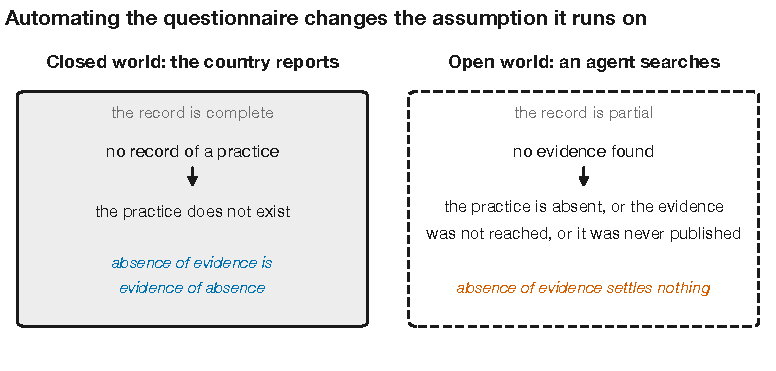
\includegraphics[width=\linewidth]{figures/fig_2_3_closed_vs_open_world.pdf}
\caption{The assumption the questionnaire runs on.}
\label{fig:assumption}
\end{figure}

Automating the questionnaire therefore changes the assumption it runs on. A country reporting on itself works under a \emph{closed world} assumption \citep{reiter1978}, where the data is full and complete, and absence of evidence of a practice equates to evidence of absence. An agent searching the open web, in the right-hand panel of Figure~\ref{fig:assumption}, has no such closure. When it finds no evidence for a practice, it cannot tell whether the practice is truly absent, or if it is just the evidence that is absent. That ambiguity makes proving a ``no'' difficult, and the system reflects this, with 87.0\% accuracy on the positive answers it commits to and 48.9\% on the negative ones (Section~\ref{sec:convergent-validity}).

\section{Approach}\label{sec:approach}

This dissertation builds and evaluates an agent swarm that answers the questionnaire from the open web. Three agents divide the work. A Researcher gathers evidence and proposes an answer. An adversarial Verifier then tries to refute that answer, searching for counterevidence, on the reasoning that opposition surfaces weak claims self-verification misses \citep{cohen2023}. Where the two cannot agree, an Adjudicator rules on the exchange. If there is an absence of substantive evidence, which may often be the case under an open world assumption, the system can also decline to answer.

The swarm is evaluated on a sample of eight of the thirty-six countries, 1,144 question-country pairs, scored against the published 2025 answers. It commits to an answer for 55.6\% of questions, agreeing with the key on approximately 70\% of those, and abstains on the remaining 44.4\%. Adding multiple agents roughly doubles the proportion of questions answered, with the number of correct answers improving similarly (Section~\ref{sec:ablation}). The premise that adversarial verification would perform better than a corroborative check did not hold. Changing the Verifier's stance leaves the results largely unchanged, consistent with recent literature. The benefit of debate appears to stem from an increased number of reasoning calls rather than from distinct stances, and varying the model may be more influential than varying the prompts \citep{chowdhury2026,zhu2026}. What bounds the system sits upstream of both, in what the open web holds, and no verifier can recover evidence that was never published. Consequently, its usefulness varies across the questionnaire, and Section~\ref{sec:reformulation} outlines a possible reformulation of the ODMI to facilitate the transition to automation.


\section{Research Questions}\label{sec:research-questions}

RQ1: Can an automated assessment meet the conditions that keep it legitimate?

RQ2: Is a swarm of agents with distinct roles more reliable in open-web retrieval than sole agents, and specifically, what is the added value of Adversarial Verification?

RQ3: What follows for the assessment itself? How much of the questionnaire can be delegated to the machine as it stands, and would the questionnaire have to be rewritten for the rest to be answerable from outside?


\section{Contributions}\label{sec:contributions}

The work makes four contributions. First, it assembles six criteria for judging a generative system that stands in for a human assessor. No framework for this yet exists \citep{unece2025}, so the criteria are drawn from a quality framework for statistical algorithms \citep{yung2022} and one for automated scoring \citep{williamson2012}, adapted to a system that also retrieves evidence. Second, it implements and documents a three-agent swarm that answers a policy assessment end-to-end, keeping a complete set of receipts for reproduction. Third, it reports an empirical test of adversarial debate where evidence is sparse, finding that the verification layer raises the share of questions answered from 26.6\% to 55.6\% whilst holding accuracy constant, and that what limits the system is the evidence the open web holds rather than the reasoning applied to it. Fourth, it turns towards the assessment, proposing how it could be reformulated to both be answerable from the web, whilst also becoming a better assessment of openness.

\section{Report Structure}\label{sec:report-structure}

Chapter~\ref{ch:background} introduces the index as a testbed, sets out the six criteria, and reviews the work on agentic retrieval, verification and abstention that the design draws on. Chapter~\ref{ch:methodology} describes the architecture and the evaluation design. Chapter~\ref{ch:results} reports the results from running the swarm through eight countries, taking the six criteria in turn. Chapter~\ref{ch:discussion} interprets the results, works through what can be delegated to an automated system, and develops the reformulation. Chapter~\ref{ch:conclusion} concludes.
